\section{Custom Action Sampling Distributions}

\label{sec:system}
When collecting data by sampling from simple distributions, such as a multivariate Gaussian, the skills that emerged were found to be generally restricted to pushing and dragging objects. This is because with simple distributions, it is very unlikely to visit states like picking up and placing of objects or folding cloth. Not only would the model be imprecise for these kinds of states, but also during planning it would be unlikely to \emph{find} action sequences that grasp an object or fold an item of clothing.
We therefore explore how the sampling distribution used both in data collection and sampling-based planning can be changed to visit these, otherwise unlikely, states more frequently, allowing more complex behavior to emerge. 

To allow picking up and placing of objects as well as folding of cloth to occur more frequently, we incorporate a simple ``reflex'' during data collection, where the gripper automatically closes, when the height of the wrist above the table is lower than a small threshold. This reflex is inspired by the palmar reflex observed in infants~\cite{grasping_fetal}. With this primitive, when collecting data with rigid objects about 20\% of trajectories included some sort of grasp. For deformable objects such as towels and cloth, this primitive helps increasing the likelihood of encountering states where cloths are folded. We found that the primitive can be slightly adapted to avoid cloths becoming tangled up. More details are provided in Appendix \ref{sec:folding_sampling}.

It is worth noting that, other than this reflex, no grasping-specific or folding-specific engineering was applied to the policy, allowing a joint pushing, grasping and folding policy to emerge through planning (see figure \ref{fig:push_grasp} in the appendix). In our experiments, we evaluate our method using data obtained both with and without the grasping reflex, evaluating both purely non-prehensile and combined prehensile and non-prehensile manipulation.

\section{Multi-View Visual MPC}
\label{sec:multiview}
\begin{wrapfigure}{r}{.45\columnwidth}
	\centering
	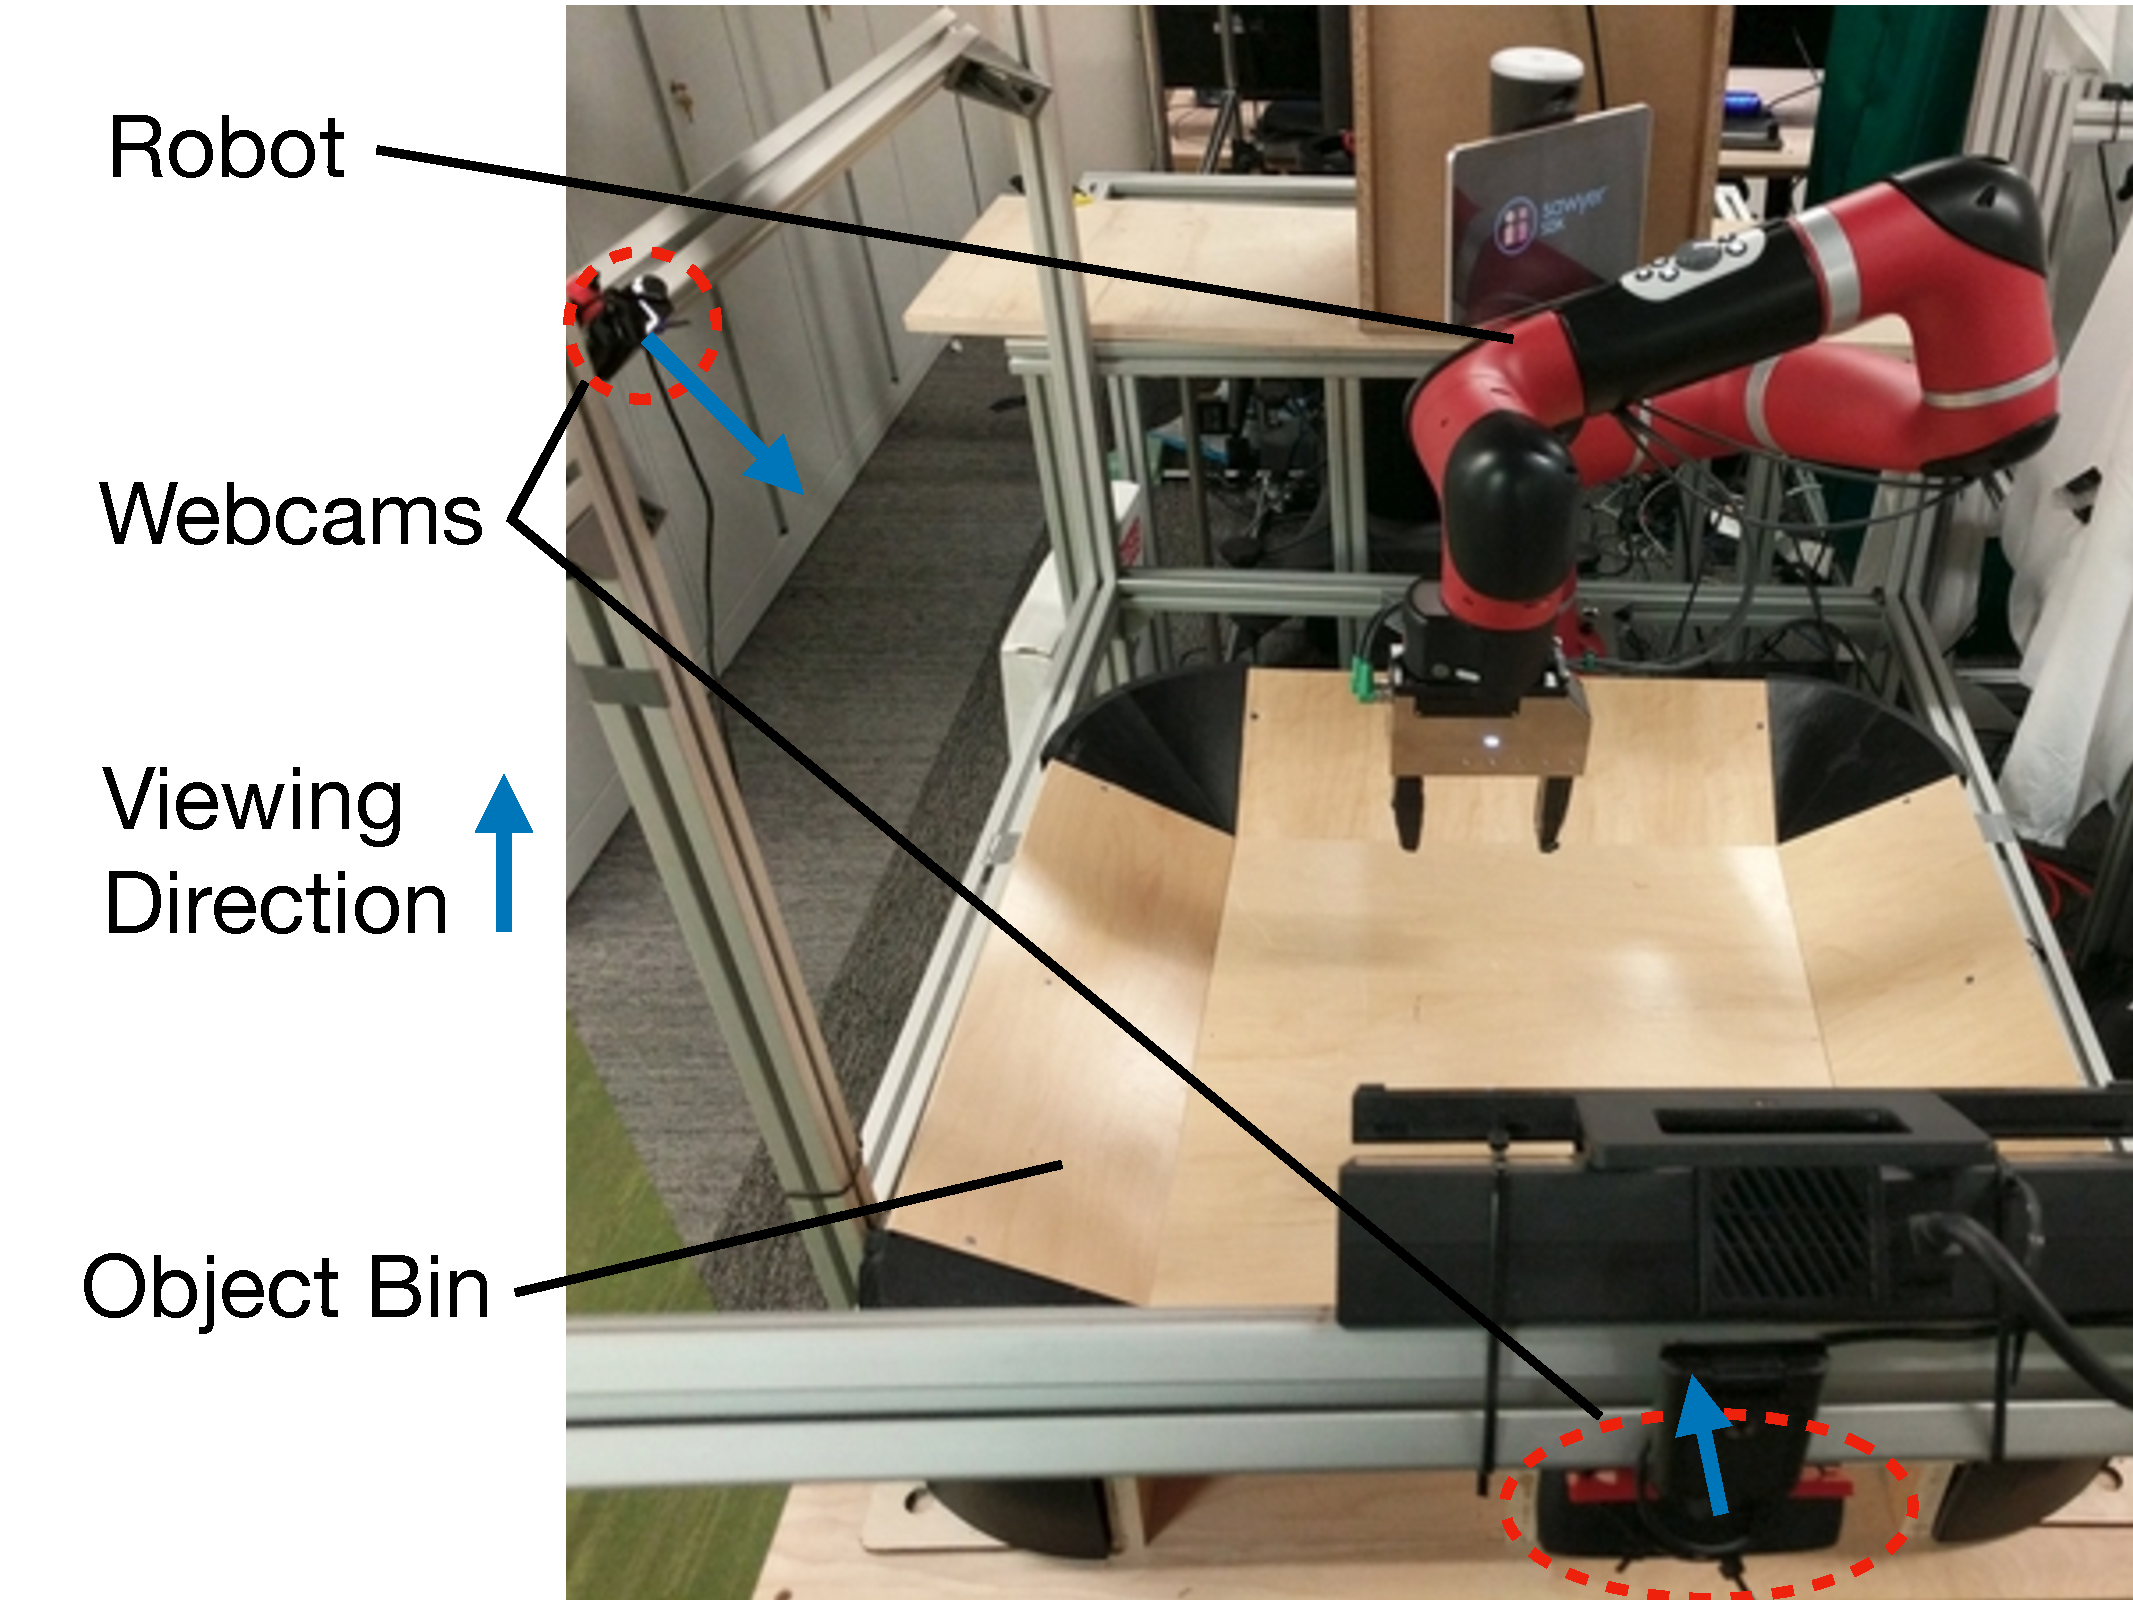
\includegraphics[width=0.45\columnwidth]{images_general/robot_setup_scheme.pdf}
	\caption{\small{Robot setup, with 2 standard web-cams arranged at different viewing angles.}}	\label{fig:robot_setup}
\end{wrapfigure}

The visual MPC algorithm as described so far is only able to solve manipulation tasks specified in 2D, like rearranging objects on the table. However, this can impose severe limitations; for example, a task such as lifting an object to a particular position in 3D cannot be fully specified with a single view, since it would be ambiguous. 
We use a combination of two views, taken from two cameras arranged appropriately, to jointly define a 3D task. Figure \ref{fig:robot_setup} shows the robot setup, including two standard webcams observing the workspace from different angles. The registration method described in the previous section is used separately per view to allow for dynamic retrying and solving temporally extended tasks. The planning costs from each view are combined using weighted averaging where the weights are provided by the registration network (see equation \ref{eqn:cost_avg}). The the first two rows of figure \ref{fig:tile_2} show a 3D object positioning task, where an object needs to be positioned at a particular point in 3D space. This task needs two views to be fully specified.





